\documentclass[tikz,border=5pt]{standalone}
\usepackage{graphicx}
\usepackage{tikz}
\usetikzlibrary{arrows.meta, positioning, backgrounds, calc}

\begin{document}
\begin{tikzpicture}[
  font=\sffamily,
  node distance=1.8cm and 1.8cm,
  >=Stealth,
  every node/.style={align=center}
]

% -- 1) Input image node --
\node (input) {\includegraphics[width=3cm]{gulls.jpg}};

% -- 2) CNN block --
\node[draw, thick, rounded corners,
      minimum width=1.8cm, minimum height=1.2cm,
      right=of input] (cnn) {\textbf{CNN}};
\draw[->, thick] (input.east) -- (cnn.west);

% -- 3) "Set of image features" block --
\node[draw, thick, rounded corners,
      minimum width=2.0cm, minimum height=1.2cm,
      right=of cnn] (features) {Set of \\ image features};
\draw[->, thick] (cnn.east) -- (features.west);

% -- 4) Transformer encoder-decoder --
\node[draw, thick, rounded corners,
      minimum width=2.0cm, minimum height=1.2cm,
      right=of features] (transformer) {Transformer\\encoder-decoder};
\draw[->, thick] (features.east) -- (transformer.west);

% -- 5) Set of box predictions (colored rectangles) --
\node[right=of transformer] (predictions) {%
  \begin{tikzpicture}[x=1.1em, y=1.1em]
    \node[draw, thick, fill=black,
          label=right:{\scriptsize no object}] (b1) at (0, 2.5) {};
    \node[draw, thick, fill=pink]   (b2) at (0, 1.5) {};
    \node[draw, thick, fill=blue]   (b3) at (0, 0.5) {};
    \node[draw, thick, fill=orange] (b4) at (0, -0.5) {};
    \node[draw, thick, fill=green]  (b5) at (0, -1.5) {};
  \end{tikzpicture}\\[3pt]
  \small Set of \\ box predictions
};
\draw[->, thick] (transformer.east) -- (predictions.west);

% -- 6) Two side-by-side matched bounding boxes images --
\node[above right=2.2cm and 2.5cm of predictions, anchor=north west] (matched2) {%
  \begin{tikzpicture}[
    % Use a consistent pixel → cm scale for the bounding boxes
    x={3cm/1344},
    y={1.71cm/768},
    anchor=north west,
    font=\sffamily
  ]

    %---------------------------------------------------------
    % FIRST (LEFT) IMAGE
    %---------------------------------------------------------
    % Place the left image so bounding boxes appear within it
    \node[inner sep=0, anchor=north west] (leftImgNW) at (0,500)
      {\includegraphics[width=3cm]{gulls.jpg}};
    
    % Define bounding boxes for the gulls (approx positions)
    % Left gull: (460,200) -> (620,340)
    \coordinate (leftBox1NW) at (460,200);
    \coordinate (leftBox1SE) at (620,340);
    \draw[line width=2pt, color=red]
      (leftBox1NW) rectangle (leftBox1SE);

    % Right gull: (680,120) -> (920,300)
    \coordinate (leftBox2NW) at (680,120);
    \coordinate (leftBox2SE) at (920,300);
    \draw[line width=2pt, color=blue]
      (leftBox2NW) rectangle (leftBox2SE);

    %---------------------------------------------------------
    % SECOND (RIGHT) IMAGE
    %---------------------------------------------------------
    % Shift everything by +1344 px horizontally so it sits to the right
    \pgfmathsetmacro{\shiftX}{1344} % image width in px
    \pgfmathsetmacro{\gap}{50}      % extra gap in px between images

    \node[inner sep=0, anchor=north west] (rightImgNW) at (\shiftX+\gap, 500)
      {\includegraphics[width=3cm]{gulls.jpg}};
    
    % Duplicate the bounding boxes in the right image
    \coordinate (rightBox1NW) at (\shiftX+\gap+460, 200);
    \coordinate (rightBox1SE) at (\shiftX+\gap+620, 340);
    \draw[line width=2pt, color=red]
      (rightBox1NW) rectangle (rightBox1SE);

    \coordinate (rightBox2NW) at (\shiftX+\gap+680, 120);
    \coordinate (rightBox2SE) at (\shiftX+\gap+920, 300);
    \draw[line width=2pt, color=blue]
      (rightBox2NW) rectangle (rightBox2SE);

    %---------------------------------------------------------
    % CONNECT corresponding bounding boxes with black arrows
    % We'll connect the centers of each rectangle
    %---------------------------------------------------------
    % Center of leftBox1
    \coordinate (leftBox1C) at ($(leftBox1NW)!0.5!(leftBox1SE)$);
    % Center of leftBox2
    \coordinate (leftBox2C) at ($(leftBox2NW)!0.5!(leftBox2SE)$);

    % Center of rightBox1
    \coordinate (rightBox1C) at ($(rightBox1NW)!0.5!(rightBox1SE)$);
    % Center of rightBox2
    \coordinate (rightBox2C) at ($(rightBox2NW)!0.5!(rightBox2SE)$);

    % Draw arrows
    \draw[->, thick, color=black] (leftBox1C) -- (rightBox1C);
    \draw[->, thick, color=black] (leftBox2C) -- (rightBox2C);

  \end{tikzpicture}
};

% Dashed arrow from predictions to the left (first) subimage
\draw[dashed,->, thick]
  (predictions.east) .. controls +(+1,0) .. (matched2.west);

% -- 7) Bipartite graph matching (during training) --
\node[right=3.5cm of predictions, yshift=1.0cm] (matchingLabel)
      {\textbf{Bipartite Matching Loss}};

\node[below=0.5cm of matchingLabel] (bipartite) {%
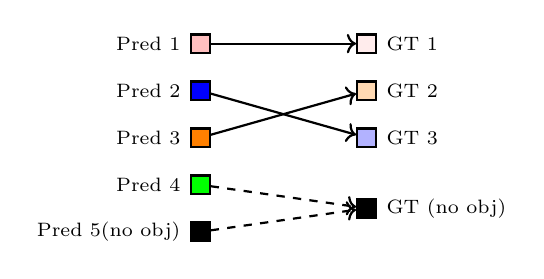
\begin{tikzpicture}[x=2.0em, y=1.7em, font=\scriptsize]
  % Predicted boxes (left side)
  \node[draw, thick, fill=pink,   label=left:Pred 1] (p1) at (0, 1) {};
  \node[draw, thick, fill=blue,   label=left:Pred 2] (p2) at (0, 0) {};
  \node[draw, thick, fill=orange, label=left:Pred 3] (p3) at (0, -1) {};
  \node[draw, thick, fill=green,  label=left:Pred 4] (p4) at (0, -2) {};
  \node[draw, thick, fill=black,  label=left:{Pred 5 \\ (no obj)}] (p5) at (0, -3) {};

  % Ground truth boxes (right side)
  \node[draw, thick, fill=pink!30,   label=right:GT 1] (gt1) at (3, 1) {};
  \node[draw, thick, fill=orange!30, label=right:GT 2] (gt2) at (3, 0) {};
  \node[draw, thick, fill=blue!30,   label=right:GT 3] (gt3) at (3, -1) {};

  % New GT (no obj) box in black
  \node[draw, thick, fill=black, label=right:{GT (no obj)}] (gtNoObj) at (3, -2.5) {};

  % Edges: matched pairs
  \draw[->, thick] (p1) -- (gt1);
  \draw[->, thick] (p2) -- (gt3);
  \draw[->, thick] (p3) -- (gt2);

  % Connect p4 and p5 to "GT (no obj)"
  \draw[dashed, ->, thick] (p4) -- (gtNoObj);
  \draw[dashed, ->, thick] (p5) -- (gtNoObj);
\end{tikzpicture}
};

\end{tikzpicture}
\end{document}
